  \mysection{The Sellsword}{trope-sellsword}

  \flavor{
    How heavy this axe \\
    Burden carried from birth \\
    Wrought in Stygian visions \\
    By the gods of the earth \\
    \Tilde The Sword, "How Heavy this Axe"
  }

  \mysubsection{The Basics}{sellsword-basics}

  \myhighlight{Tough}{sellsword-flesh}
  
  Sellswords have a d10 \FLESH


  \myhighlight{Fortitude}{sellsword-fortitude}
  
  You add your \LVL to any \RO or \RB attempt that includes your \VIG die.  

  \myhighlight{The Deed Die}{sellsword-deed-die} 

  You start with a d4 Deed Die, a \UD whose result can be applied to any of your Fight checks. 

  Roll the Deed Die and add its result to your Fight roll; if you hit, also add the result to your damage (applied \mybold{after} the die explodes, if applicable).  You can roll your Deed Die \myital{after} your Fight check is rolled (it doesn't have to be at the same time), but you can only roll it once per Moment.  Don't forget that this is a \UD, so it moves \DCDOWN if you roll a 1 or a 2.
  


  \begin{center}
  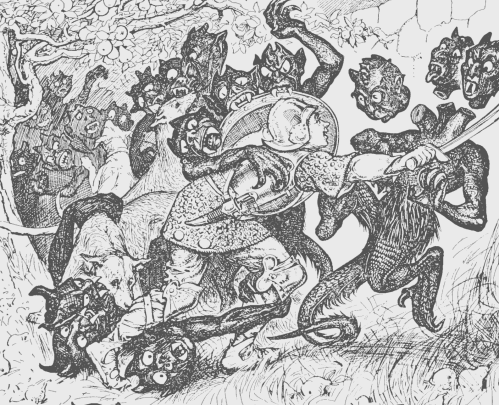
\includegraphics[scale=.4]{Sellsword_1}
  \end{center}


  \mysubsection{Creation}{sellsword-creation}

  \callout{
    \mynumlist {
      \item Move any of your core Skills \DCUP
      \item Move any of your core Saves \DCUP
      \item Give yourself a Deed Die of d4
      \item Pick \mybold{three} \mylink{Virtues}{sellsword-virtues} from the list below.  You can only pick each Virtue once.
      \item Pick \mybold{one} \mylink{Complication}{sellsword-complications} from the list below (or make up your own with the Arbiter!)
      \item Write down your Starting Gear
    }
  }


    \mytable{X}{
      \thead{\mysubsection{Virtues}{sellsword-virtues}} \\
    }{ 
      \mylink{Blademaster}{sellsword-virtue-blademaster} \\
      \mylink{Duelist}{sellsword-virtue-duelist} \\
      \mylink{Huntsman}{sellsword-virtue-huntsman} \\
      \mylink{Intangibles}{sellsword-virtue-intangibles} \\
      \mylink{Lethal}{sellsword-virtue-lethal} \\
      \mylink{My Father's Sword}{sellsword-virtue-fathers-sword} \\
      \mylink{Second Skin}{sellsword-virtue-second-skin} \\
      \mylink{Three Kills Per Stroke}{sellsword-virtue-three-kills} \\
      \mylink{Tougher Than a Coffin Nail}{sellsword-virtue-coffin-nail} \\
      \mylink{Veteran}{sellsword-virtue-veteran} \\
    }

    \myhighlight{Blademaster}{sellsword-virtue-blademaster}

    Two handed weapons count as one Significant Item instead of two. You also add your \LVL to damage (applied \mybold{after} the die explodes, if applicable)

    \myhighlight{Duelist}{sellsword-virtue-duelist}

    You start the game with two Fast weapons of your choice (including the Knave's Sword).  You can use the Florentine Mighty Deed regardless of your \DEX

    \myhighlight{Huntsman}{sellsword-virtue-huntsman}

    You start the game with Light Armor and a Strongbow with a Quiver of Arrows (d10 \UD)

    \myhighlight{Intangibles}{sellsword-virtue-intangibles}

    You may move two different Intangible Stats of your choice \DCUP.  Describe to the Arbiter why these Intangible Stats are better than average.

    \myhighlight{Lethal}{sellsword-virtue-lethal}

    If you roll \MAX damage for your weapon, the die explodes i.e. you roll again and add the second roll to the first.  If you roll \MAX damage again, the roll continues.  This roll has to be a \myital{natural} (not modified) roll (though some powers and abilities can change a natural roll).  Modifiers to damage are added or subtracted  \mybold{after}  the die explodes (including Deed Die).  Note that this means you can't \mylink{Crit}{combat-crits-and-fumbles} since your last roll is never technically the \MAX. 

    \example{Charse the Lethal attacks a goblin with a Shortsword (d6).  He makes his Fight check and hits, and rolls a 6 for damage. He rolls again and rolls another 6.  He rolls a 3rd time and rolls a 4.  He deals 16 points of damage(!) [6+6+4] and the goblin is reduced to a fine pink mist.}


    \myhighlight{My Father's Sword}{sellsword-virtue-fathers-sword}

    You start the game with a Hard Brawl weapon of your choice.  With this weapon \mybold{only} your Fight \RO is +4, your damage explodes as if you had the Trait \mylink{Lethal}{sellsword-virtue-lethal}, and you cannot be Disarmed. If you lose this weapon, you lose the abilities that go with it.  You have to describe to the Arbiter what makes this weapon unique.

    \myhighlight{Second Skin}{sellsword-virtue-second-skin}

    Your armor doesn't count as a Significant Item.  You can repair 1 \UD of your Armor when you take a \mylink{Breather}{combat-resting-breather}, 
    up to its \MAX \UD.   You start the game with a suit of Light or Medium Armor.  The Armor should look unique; describe what it looks like to the Arbiter.

    \myhighlight{Three Kills Per Stroke}{sellsword-virtue-three-kills}
    
    Treat any Brawl weapon you use as if it had Cleave.

    \cbreak

    \myhighlight{Tougher Than a Coffin Nail}{sellsword-virtue-coffin-nail}

    Immediately:
    \dashedbox {
    \mybullet {
        \item Raise any of your Saves \DCUP (this is in addition to your initial Save \DCUP);
        \item Raise your \DEATH to start at \mybold{Tough, d12}
        \item Add +2 Flesh
    }}

    Every time you gain a level:  roll your \VIG.  If the result of your roll is greater than your current Flesh, replace your Flesh with that result.  You can make this roll at any time during Vacation.

    \example{Charse the Tough currently has 12 Flesh, and hits level 2.  He chooses to advance his \VIG to d12, then opts to roll for his new Flesh.  He rolls a d12 and adds his \LVL (since he's rolling his Primary Stat), getting a 13.  Nice.  He now has 13 Flesh)}

    \myhighlight{Veteran}{sellsword-virtue-veteran}

    You have some experience with a prior \mylink{Band}{the-band}.  You start with d6+1 Grit.  Tell the Arbiter the name of your old \mylink{Band}{the-band}, and what happened to them.


    \newpage


    \mytable{X}{
      \thead{\mysubsection{Complications}{sellsword-complications}} \\
    }{
      Alcoholic \\
      Cheap Tricks \\
      The Cimmerian \\
      Credo \\
      Filthy \\
      Hippophobia \\
      Honorable \\
      Mortal Enemy \\
      Pit Fighter \\
      Sins of the Father \\
    }

    \myhighlight{Alcoholic}{sellsword-complication-alcoholic}

    You are addicted to alcohol.  Whenever you take a Breather, you have to take a drink or you heal no Grit.  \RS your \VIG when you do - if you Fail, you gain 1 point of \mylink{Drunk}{effect-drunk}. 

    When you take a Bivouac, you must roll a \UD for an alcoholic beverage, or you gain none of the beneficial effects. \RS your \VIG at the end of the Bivouac - if you fail, you are \mylink{Hung Over}{effect-hung-over}


    \myhighlight{Cheap Tricks}{sellsword-cheap-tricks}

    You do not like or trust magic, \mylink{Philosophers}{trope-philosopher}, or the unnatural (including \mylink{The Unseelie}{unseelie}).  The degree to which you feel this way is up to you.  Let the Arbiter know why.

    \myhighlight{The Cimmerian}{sellsword-complication-cimmerian}

    Your appearance is so outlandish even educated and well-traveled people will stop to stare at you. People can pick you easily out of a crowd, and your reputation precedes you.

    \myhighlight{Credo}{sellsword-complication-credo}
  
    You must make a vow - a short, specific, personal statement that you will not forget. For example, "I will protect my friend Johann" or "I will never harm an unarmed person".  You must follow this vow to the best of your ability

    \myhighlight{Filthy}{sellsword-complication-filthy}

    You refuse to bathe except under the most dire circumstances.  Your general hygiene is horrible.  You can never use your Presence to charm someone (intimidate is a different story), and if you're downwind from Monsters it might affect your ability to surprise them.

    \myhighlight{Hippophobia}{sellsword-complication-hippophobia}

    You are afraid of horses and mules.  You refuse to ride one (riding in a cart is OK).


    \myhighlight{Honorable}{sellsword-complication-honorable}

    You refuse payment for good deeds, always rescue the helpless, and refuse to fight unarmed foes (within reason, of course).  

    \myhighlight{Mortal Enemy}{sellsword-complication-mortal-enemy}

    You have a mortal enemy, someone powerful who has done you significant wrong.  This enemy should be substantially more powerful than you.  You are driven by your revenge against this mortal enemy. Tell the Arbiter who they are, and why they are your enemy.

    \myhighlight{Pit Fighter}{sellsword-complication-pit-fighter}

    You strongly believe that combat should take place between two people face-to-face.  You won't use Shoot weapons, and you'll never throw a Throw weapon at a target.

    \myhighlight{Sins of the Father}{sellsword-complication-sins-father}

    Your parent (alive or dead) is infamous.  If people ever discover that you are their child, they will have significant negative reactions.  At the Arbiter's complete discretion you will encounter various assassins, sellswords, and kidnappers who have figured out who you are, and want to do you harm.  Tell the Arbiter a bit about this parent.


  \mysubsection{Starting Gear}{sellsword-starting-gear}

  \mybullet {
    \item 2 iron pieces; 
    \item a backpack containing a worn bedroll;
    \item d4 \UD of personal provisions;
    \item a stained and patched waterproof cloak;
    \item a pitted shield, rusty helmet, and sharpened spear
    \item one pick OR 3 rolls on the \mylink{Random Items}{appendixb-random-items} table in Appendix B;
  }   


    \mysubsection{Examples}{sellsword-examples}

    \myhighlight{The Old Campaigner}{sellsword-soldier}

    \example{Travel, Veteran, Second Skin, My Father's Sword, Credo}

    \myhighlight{The Barbarian}{sellsword-barbarian}

    \example{Bushcraft, Tougher Than a Coffin Nail, Three Kills Per Stroke, Lethal, The Cimmerian}

    \cbreak\bump

    \myhighlight{The Sword Saint}{sellsword-sword-saint}

    \example{Listen, Blademaster, Lethal, Duelist, Alcoholic} 
    
    \myhighlight{The Ranger}{sellsword-ranger}

    \example{Bushcraft, Veteran, Lethal, Huntsman, Honorable}

